\documentclass[12pt,a4paper,draft]{ctexart}
\usepackage[utf8]{inputenc}
\usepackage{amsmath}
\usepackage{amsfonts}
\usepackage{amssymb}
\usepackage{graphicx}
\usepackage{bm}
\usepackage{booktabs}
\usepackage[backend=biber,backref=true%nature,% citestyle=gb7714−2015,backref=true%
]{biblatex}
%参考文献数据源加载 
\addbibresource[location=local]{ref.bib}
%\usepackage[left=3.0cm, right=3.0cm, top=3.5cm, bottom=2.70cm]{geometry}
\title{隐马尔科夫模型 \\
	在拼音输入法中的应用研究}
\author{Yuan}
\date{\small\today}
\begin{document}

\maketitle
\begin{abstract}
本文尝试将隐马尔科夫模型应用于中文整句拼音输入中,给出了具体的模型和实际问题的对应关系以及参数估计的方法。同时还选用了现有的中文语料库进行了实现,取得了较好的效果。
\end{abstract}	
\section{引言}
隐马尔科夫模型(Hidden Markov Model,HMM)是一种应用于序列问题的统计学系模型,该模型描述了由隐藏的马尔科夫链随机生成观测序列的过程。HMM非常适合解决标注问题,故HMM在语音识别、自然语言处理、生物信息、模式识别等领域有广泛的应用,本文着眼于将HMM应用于中文拼音输入法。拼音输入法将拼音转换为对应汉字,其中更具有实用价值的是将连续的拼音输入转换为连续的句子。这是典型的序列问题,更为具体地,是一种序列标注问题,故应用HMM能较好的解决该问题。
\section{问题描述}
HMM描述了一个隐藏的马尔科夫链生成不可观测的状态随机序列,再由各个状态生成一个观测而产生观测随机序列的过程。HMM随机生成的状态序列成为状态序列(state sequence);每一个状态生成一个观测,而由此产生的观测的随机序列成为观测序列(observation sequence)。故HMM可以由初始概率分布、状态转移概率分布以及观测概率分布确定,这三者对应的参数分别为初始状态概率向量$ \bm{\pi} $、状态转移概率矩阵$\bm{A}$及观测概率矩阵$\bm{B}$。由此HMM可以用三元组$ \lambda=(\bm{A},\bm{B},\bm{\pi}) $表示\cite{李航统计学习}。
\subsection{模型定义}
在拼音序列转汉字的问题中,连续的句子被视为序列,即认为每个时刻对应一个汉字,汉字又对应拼音。由于用户在输入法中输入的是拼音,所以拼音序列被定义为观测序列。而汉字则为生成观测序列的状态序列。故本应用下的HMM相关定义为:


所有的汉字组成集合Q(状态集合),所有汉字对应的拼音的集合V(观测集合),其中$ |Q|=N, |V|=M $。
\[ Q=\{ \mbox{汉字}_1,\mbox{汉字}_2,\cdots,\mbox{汉字}_N \},V=\{ \mbox{拼音}_1,\mbox{拼音}_2,\cdots,\mbox{拼音}_M \}  \]

用户想输入的汉字序列I(状态序列),用户实际输入的拼音序列O(观测序列),其中$ |I|=|O|=T $。
\[ I=\{ \mbox{预期汉字}_1,\mbox{预期汉字}_2,\cdots,\mbox{预期汉字}_T \}	\]
\[O=\{ \mbox{输入拼音}_1,\mbox{输入拼音}_2,\cdots,\mbox{输入拼音}_T \}  \]

句子中前后汉字转移概率矩阵$\bm{A}$:
\[ \bm{A}=[a_{ij}]_{N\times N} \]
其中,
\[ a_{ij}=P(i_{t+1}=\mbox{汉字}_j|i_t=\mbox{汉字}_i),  i=1,2,3,\cdots,N; j=1,2,\cdots,N\]
是在句子中的位置$ t $处的$ \mbox{汉字}_i $转移到$ t+1 $处的$ \mbox{汉字}_j $的概率。
句子中前后汉字转移概率矩阵$\bm{B}$:
\[ \bm{B}=[b_j(k)]_{N\times M} \]
其中,
\[ b_j(k)=P(\mbox{t处输入的拼音}=\mbox{拼音}_k|\mbox{ t处想要输入的汉字}=\mbox{汉字}_j) \]
\[ k=1,2,3,\cdots,M; j=1,2,\cdots,N\]
是在句子中的位置$ t $处的$ \mbox{汉字}_j $生成$ \mbox{拼音}_k $的概率。

句子中首个汉字出现可能性的概率向量$\bm{\pi}$:
\[ \bm{\pi}=(\pi_i) \]
其中,
\[ \pi_i=P(\mbox{句首汉字}=\mbox{汉字}_i), i=1,2,\cdots,N \]
是句首汉字为$\mbox{汉字}_i$的概率。
\subsection{模型训练(参数估计)}
HMM的训练可以采用监督学习或者无监督学习\cite{李航统计学习},本应用的状态和观测为汉字和拼音。将汉字转化为拼音可以自动开展\cite{python-pinyin},并有相当高的准确度\cite{accuracy-of-auto-pinyin}。故可以通过中文语料库生成用于监督学习的训练集。
本应用中HMM的三元组$ \lambda=(\bm{A},\bm{B},\bm{\pi}) $的估计方法如下:
\paragraph{前后汉字转移概率$a_{ij}$的估计}
\[ \hat{a}_{i j}=\frac{A_{ij}}{\sum_{j=1}^{N} A_{i j}}, \quad i=1,2, \cdots, N ; j=1,2, \cdots, N \]
\paragraph{汉字转拼音的概率$b_j(k)$的估计}
\[ \hat{b}_{j}(k)=\frac{B_{j k}}{\sum_{k=1}^{M} B_{j k}}, \quad j=1,2, \cdots, N ; k=1,2, \cdots, M \]
\paragraph{句首汉字出现概率$\pi_i$的估计}


\section{实验}
参数估计使用的语料源自搜狗实验室提供的搜狐往年的新闻数据集\cite{SogouCS}。原始的数据集非常庞大,通过清洗整理后得到如表x所述的数据集。


\begin{table}[]
	\begin{tabular}{@{}ll@{}}
		\toprule
		句子长度 & 平均错误率 \\ \midrule
		任意长度 & 29.7\% \\
		\textless{}=5 & 22.4\% \\
		\textgreater{}5 且 \textless{}=10 & 31.0\% \\
		\textless{}11 且 \textless{}=20 & 36.2\% \\
		\textgreater{}20 & 42.6\% \\ \bottomrule
	\end{tabular}
\end{table}


% Please add the following required packages to your document preamble:
% \usepackage{booktabs}
\begin{table}[]
	\begin{tabular}{@{}ll@{}}
		\toprule
		句子长度                             & 样例                                                                                                                                                                                                                                                                                                                                                                                                                                                                                                                                                                                                                                           \\ \midrule
		\textless{}=5                    & \begin{tabular}[c]{@{}l@{}}LEN: 2 ERROR:0.00\%\\     DIFF:  小  时\\ LEN: 5 ERROR:0.00\%\\     DIFF:  每  日  电  讯  报\\ LEN: 2 ERROR:50.00\%\\     DIFF:  万- 铢+ 株\\ LEN: 2 ERROR:0.00\%\\     DIFF:  上  周\\ LEN: 2 ERROR:0.00\%\\     DIFF:  汇  总\end{tabular}                                                                                                                                                                                                                                                                                                                                                                                   \\
		\textgreater{}5 且 \textless{}=10 & \begin{tabular}[c]{@{}l@{}}LEN: 7 ERROR:71.43\%\\     DIFF:  表  现- 得- 畏- 首- 畏- 尾+ 的+ 位+ 授+ 为+ 未\\ LEN:10 ERROR:40.00\%\\     DIFF:  公  司  法  人- 代+ 带  表- 蔡- 义- 坚+ 才+ 艺+ 建  等\\ LEN: 8 ERROR:37.50\%\\     DIFF:  将  联  合- 通- 信+ 同+ 心  产  业- 报+ 保\\ LEN: 8 ERROR:12.50\%\\     DIFF:  专  卖  店  将  不  再- 专+ 转  卖\\ LEN: 7 ERROR:42.86\%\\     DIFF:  说  不  定  能- 制- 服- 他+ 只+ 负+ 她\end{tabular}                                                                                                                                                                                                                                                 \\
		\textless{}11 且 \textless{}=20   & \begin{tabular}[c]{@{}l@{}}LEN:16 ERROR:31.25\%\\     DIFF:  柳  州  市- 阳- 光- 花+ 养+ 广+ 华  园- 游- 泳+ 有+ 用  场  有  限  责  任  公  司\\ LEN:16 ERROR:12.50\%\\     DIFF:  延  迟  等- 与+ 于  网  络  品  质  相  关  特  性  非  常  看- 重+ 中\\ LEN:12 ERROR:66.67\%\\     DIFF:- 应- 至+ 影+ 制  少- 与+ 于  一  种- 以- 上- 药- 物- 合+ 意+ 伤+ 要+ 务+ 和  用\\ LEN:11 ERROR:18.18\%\\     DIFF:- 每+ 美  外  包  一  次  就  要- 扒+ 把  一  层  皮\\ LEN:14 ERROR:42.86\%\\     DIFF:- 芷+ 之  江  西  路  街  道  会  同- 区- 城- 管- 执- 法+ 去+ 成+ 关+ 指+ 发  局\end{tabular}                                                                                                                                     \\
		\textgreater{}20                 & \begin{tabular}[c]{@{}l@{}}LEN:23 ERROR:21.74\%\\     DIFF:  在  空  调  出  风  口  下  方  还  设  计  了  一  个  抽  屉  的- 形- 式+ 行+ 驶  的- 储- 物- 格+ 出+ 无+ 个\\ LEN:26 ERROR:15.38\%\\     DIFF:  老  女  排  国- 手+ 首  周- 晓+ 小  兰- 作- 为+ 坐+ 位  本  次  中  美  女  排  超  级  对  抗  赛  的  特  邀  嘉  宾\\ LEN:25 ERROR:24.00\%\\     DIFF:  杆  进  入  最  后  一  轮  的- 伍- 兹- 毋- 庸- 置- 疑+ 物+ 资+ 无+ 用+ 职+ 仪  在  决  赛  轮  面  临  着  两  难  境  地\\ LEN:21 ERROR:76.19\%\\     DIFF:  情  况  严  重  的+ 利+ 催- 李- 翠- 琼- 被- 好- 心- 的- 路- 人- 送- 到- 中- 医- 院- 抢- 救\\ LEN:21 ERROR:14.29\%\\     DIFF:  在  用  药  过  程  中  仍- 宜+ 以  定  期  进  行  尿  常  规  和- 肾- 功+ 深+ 宫  能  测  定\end{tabular} \\ \bottomrule
	\end{tabular}
\end{table}

\begin{figure}
	\centering
	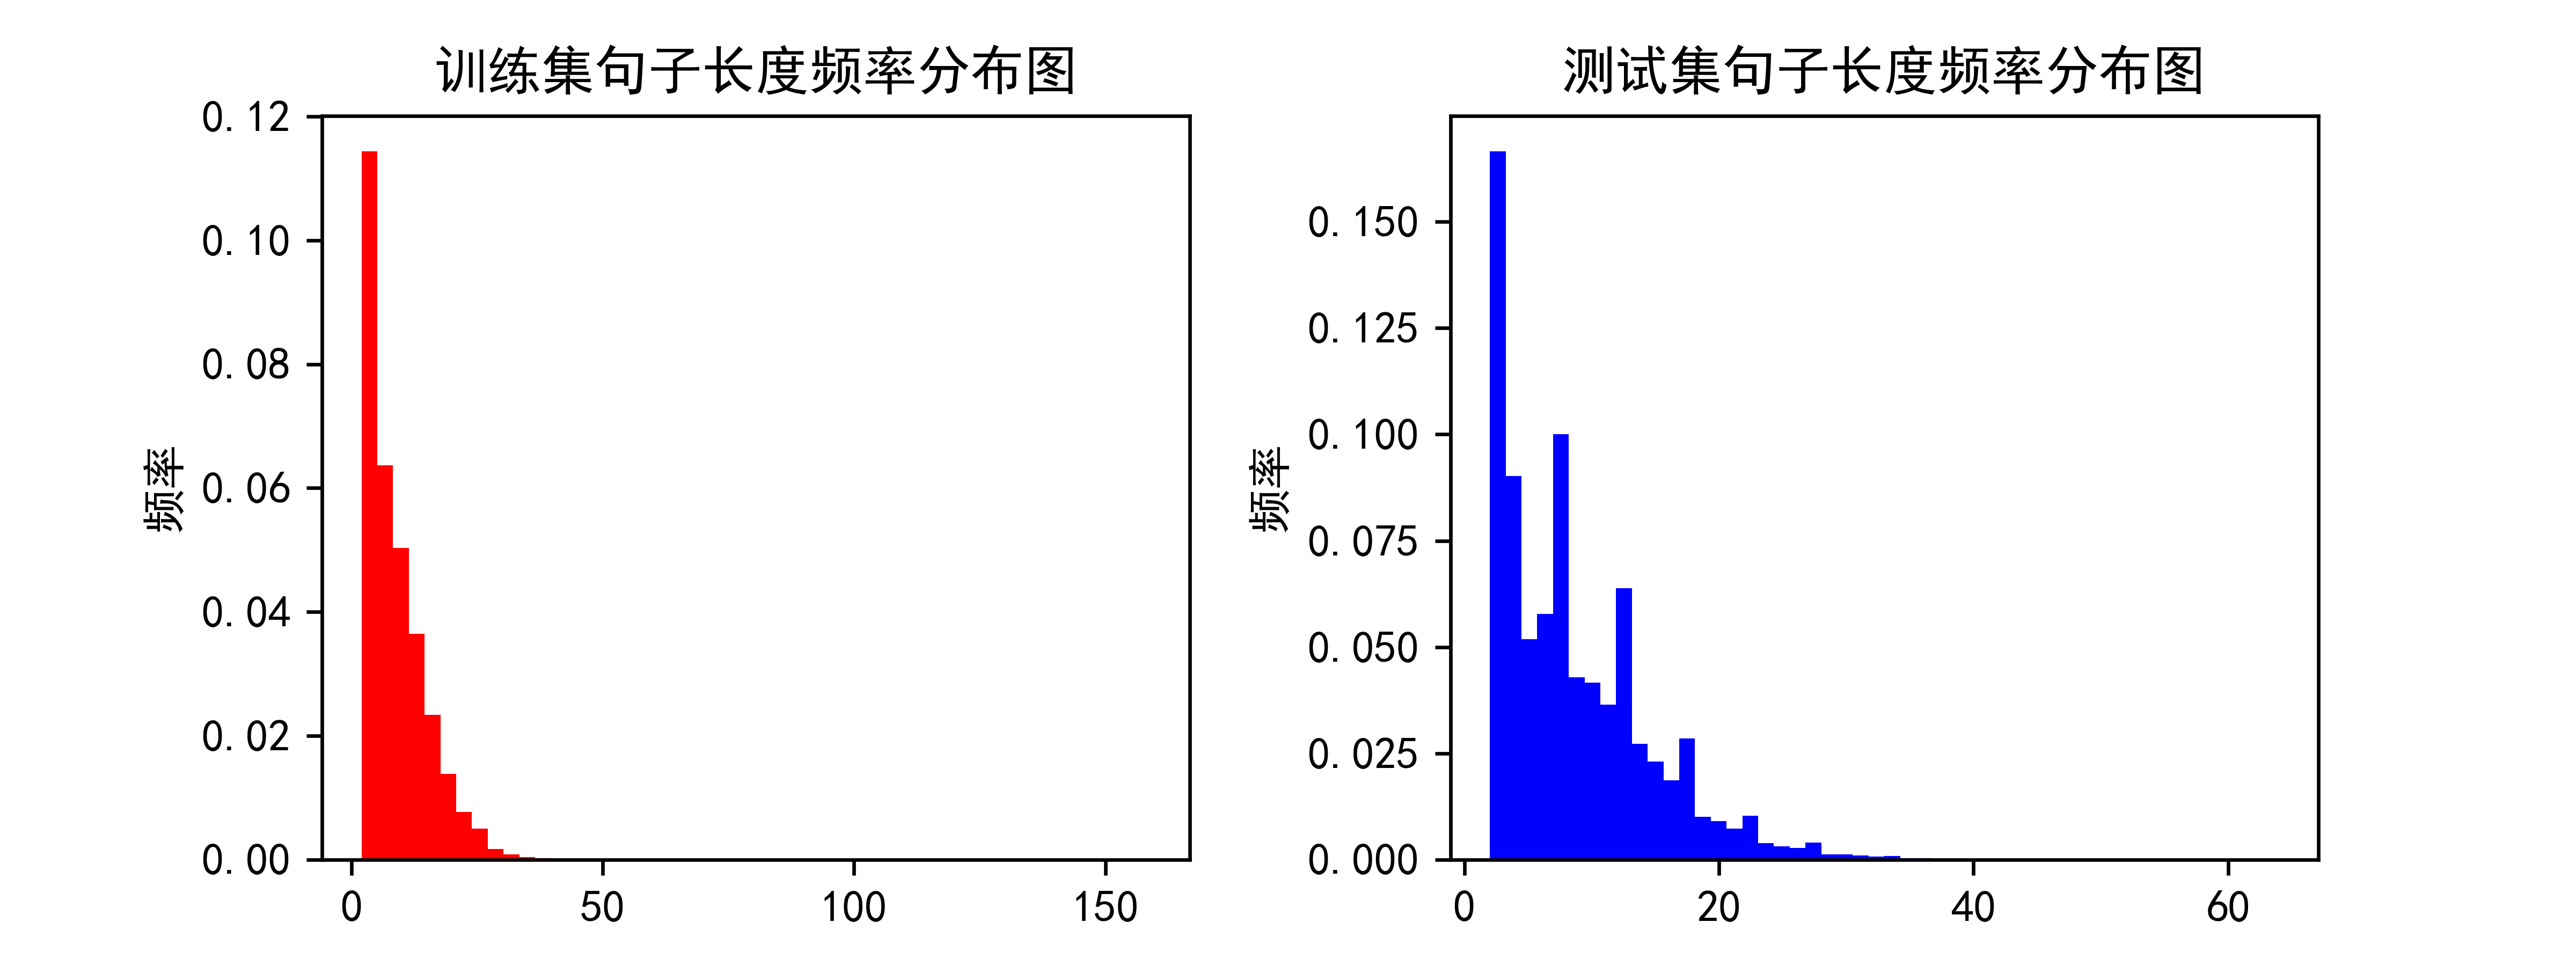
\includegraphics[width=1\linewidth]{DataSetHistogram}
	\caption{}
	\label{fig:datasethistogram}
\end{figure}




\printbibliography[heading=bibliography,title=参考文献]
\end{document}